\documentclass[12pt]{article}
\usepackage[margin=1in]{geometry}
\usepackage{amsmath,amsthm,amssymb,amsfonts}
\usepackage{bm}
\usepackage{graphicx}

\newcommand{\N}{\mathbb{N}}
\newcommand{\Z}{\mathbb{Z}}


\begin{document}


\title{Homework 4}
\author{Yasheng Sun}
\date{}

\maketitle
[This project is also available on my github https://github.com/sunyasheng/Neural-Network-Assignment]
\section{Problem Restatement}
In this assignment, the LSTM neural network will be used to deal with an emotion classification problem. Two problems are given below, the dataset used in this homework is part of the SJTU Emotion EEG Dataset (SEED), i.e. a three-class classification problem and the features extracted from emotional EEG signals. 

\subsection{Problem 1}
Building LSTM classification models individually, i.e. you are required to build one model for each of the three .npz file provided. The features from first 9 movie clips should be used as training data, and data from the rest 6 clips should be used as test data.
During watching movie clips, emotions of subjects would change with time.
  
LSTMs are suitable to capture this temporal information.
You should design the structure of the network: number of hidden layers, LSTM
time steps, batch size, epoch number, and so on.

\subsection{Problem 2}
EEG signals are different for different people, and this might cause trouble in building an universal emotion model for different people.
In this task, you are required to build an LSTM model with all .npz files provided, and compare the classification results with results in Problem 1.
The training data in this problem should be the concatenation of the training data in Problem 1, and the test data should be the concatenation of the test data in Problem 2.

\section{Solution 1}
To incorporate the temporal dependency information of features, LSTM neural networks is introduced here to as a temporal encoder. And a classifier works on top of it to classify the signals. The structure of this whole network is shown below.
\begin{center}
  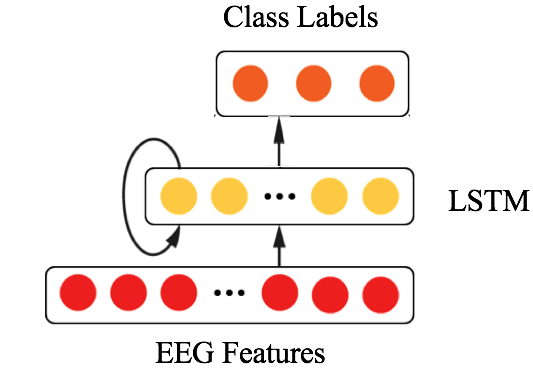
\includegraphics[angle = 0, width = .5\textwidth]{./../src/LSTMnet.png}
\end{center}
The trainning loss and validation accuracy is shown below. 
\begin{center}
  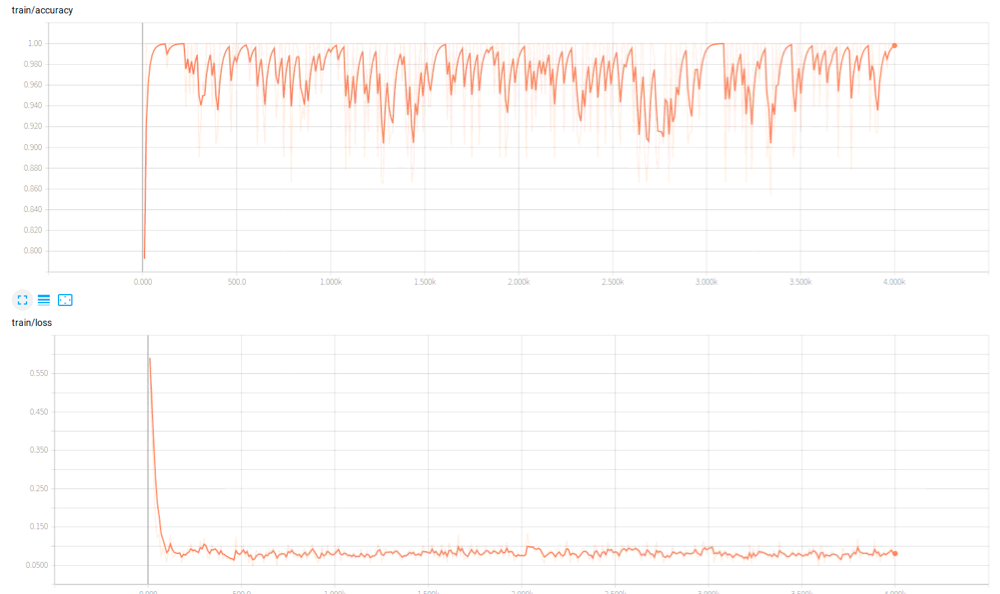
\includegraphics[angle = 0, width = .9\textwidth]{./../src/loss_accuracy.png}
\end{center}
Its corresponding hyparameter is shown below. After several training iterations, the training loss and validation accuarcy reach the optimal and begin to oscillate.\\

\begin{center}
	\begin{tabular}{|c|c|}
	LSTM hidden states & 16\\
	learning rate & 0.005\\
	dropout probability & 0.5\\
	L2 regulization & 0.5\\
	\end{tabular}
\end{center}


Following the same Hyper-parameter settings[1] in SEED dataset, we average the accuracy of 200 models using the randomly selected Hyper-parameters. The number of epoches is set to 30 and the average accuracy is 0.95445. 

\section{Solution 2}
In this section, we aim to show the difference of individuals by training a universal emotion model for all the people. With the same Hyper-parameter setting as before, the average accuracy here is 0.90729. It is lower than previous acuuracy because the distribution of data on different people are different. 

In order to further expose the patterns of these three persons, the t-sne embeddings is ploted below. The three different persons are shown with different colors. The distribution of different people is different, making an universal model perform unsatisfactory. So the domain adaption is required to match the inter-subject distribution.

\begin{center}
	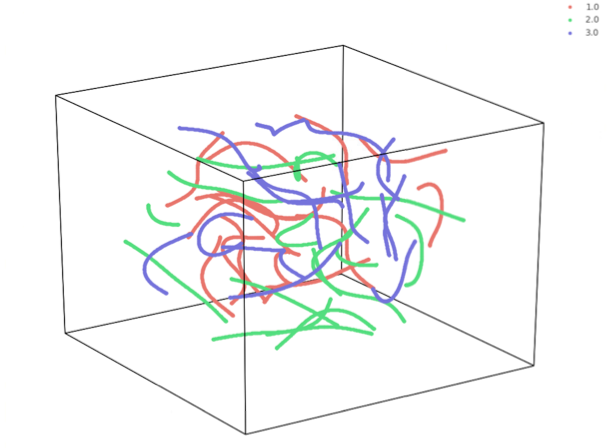
\includegraphics[angle = 0, width = .8\textwidth]{./../src/t-sne.png}
\end{center}

\section{Conclusion}
In this assignment, we classify the emotions through LSTM network successfully and show the individual difference by t-sne embedding. Modeling their emotions with a universal model is not satisfactory. Therefore, some transfer learning technique has been proposed to eliminate the inter-subject discrepancy[2]. 

\section{Reference}
\begin{flushleft}
[1]Tang, H., Liu, W., Zheng, W. L., Lu, B. L. (2017). Multimodal emotion recognition using deep neural networks.

[2]Jia-Jun Tong, Yun Luo, Bo-Qun Ma, Wei-Long Zheng, Bao-Liang Lu, Xiao-Qi Song and Shi-Wei Ma, Sleep Quality Estimation with Adversarial Domain Adaptation: From Laboratory to Real Scenario, to  appear in Proc. IJCNN’18, 
\end{flushleft}

\end{document}
